%%%%%%%%%%%%%%%%%%%%%%%%%%%%%%%%%%%%%%%%%
% Beamer Presentation
% LaTeX Template
% Version 1.0 (10/11/12)
%
% This template has been downloaded from:
% http://www.LaTeXTemplates.com
%
% License:
% CC BY-NC-SA 3.0 (http://creativecommons.org/licenses/by-nc-sa/3.0/)
%
%%%%%%%%%%%%%%%%%%%%%%%%%%%%%%%%%%%%%%%%%

%----------------------------------------------------------------------------------------
%	PACKAGES AND THEMES
%----------------------------------------------------------------------------------------

\documentclass{beamer}

\mode<presentation> {

% The Beamer class comes with a number of default slide themes
% which change the colors and layouts of slides. Below this is a list
% of all the themes, uncomment each in turn to see what they look like.

%\usetheme{default}
%\usetheme{AnnArbor}
%\usetheme{Antibes}
%\usetheme{Bergen}
%\usetheme{Berkeley}
%\usetheme{Berlin}
%\usetheme{Boadilla}
%\usetheme{CambridgeUS}
%\usetheme{Copenhagen}
%\usetheme{Darmstadt}
%\usetheme{Dresden}
%\usetheme{Frankfurt}
%\usetheme{Goettingen}
%\usetheme{Hannover}
%\usetheme{Ilmenau}
%\usetheme{JuanLesPins}
%\usetheme{Luebeck}
\usetheme{Madrid}
%\usetheme{Malmoe}
%\usetheme{Marburg}
%\usetheme{Montpellier}
%\usetheme{PaloAlto}
%\usetheme{Pittsburgh}
%\usetheme{Rochester}
%\usetheme{Singapore}
%\usetheme{Szeged}
%\usetheme{Warsaw}

% As well as themes, the Beamer class has a number of color themes
% for any slide theme. Uncomment each of these in turn to see how it
% changes the colors of your current slide theme.

%\usecolortheme{albatross}
%\usecolortheme{beaver}
%\usecolortheme{beetle}
%\usecolortheme{crane}
%\usecolortheme{dolphin}
%\usecolortheme{dove}
%\usecolortheme{fly}
%\usecolortheme{lily}
%\usecolortheme{orchid}
%\usecolortheme{rose}
%\usecolortheme{seagull}
%\usecolortheme{seahorse}
%\usecolortheme{whale}
%\usecolortheme{wolverine}

%\setbeamertemplate{footline} % To remove the footer line in all slides uncomment this line
%\setbeamertemplate{footline}[page number] % To replace the footer line in all slides with a simple slide count uncomment this line

%\setbeamertemplate{navigation symbols}{} % To remove the navigation symbols from the bottom of all slides uncomment this line
}

\usepackage[utf8]{inputenc}
\usepackage[portuguese]{babel}
\usepackage{color,soul}
\usepackage{graphicx} % Allows including images
\usepackage{booktabs} % Allows the use of \toprule, \midrule and \bottomrule in tables

%----------------------------------------------------------------------------------------
%	TITLE PAGE
%----------------------------------------------------------------------------------------

\title[Framework para Redes Sociais]{Framework para Redes Sociais baseadas em Compartilhamento de Rotas e Agendas}

\author{Álex Mesquita \& Jefferson Xavier}

\institute[UnB]
{
\textit{alex.mesquita0608@gmail.com}
\textit{jeffersonx.xavier@gmail.com}\\
Universidade de Brasília\\
\medskip
}
\date{15 de Dezembro de 2015}

\begin{document}

\begin{frame}
\titlepage
\begin{center}
Orientadores\\
Prof. Dr. Maurício Serrano\\
Prof. Dr. Milene Serrano
\end{center}
\end{frame}

\begin{frame}
\frametitle{Visão Geral}
\tableofcontents
\end{frame}

%----------------------------------------------------------------------------------------
%	PRESENTATION SLIDES
%----------------------------------------------------------------------------------------

\section{Contextualização}

\begin{frame}
\frametitle{Contextualização}

\begin{itemize}
\item Reutilização de Software;
	\begin{itemize}
		\item Processo de criar sistemas de software a partir de um software já existente \cite{krueger}.
	\end{itemize}
\item Redes Sociais.
	\begin{itemize}
		\item Conjunto de participantes unindo ideias e recursos em torno de relacionamentos, valores e interesses compartilhados \cite{marteleto}.
	\end{itemize}
\end{itemize}

\begin{figure}[h]
	\centering
	\includegraphics[scale=0.45]{figuras/social_network.eps}
\end{figure}

\end{frame}

\section{Motivação}

\begin{frame}
\frametitle{Motivação}

\begin{itemize}
	\item Ideia inicial para \textbf{redes sociais generalizadas};
	\item Problema com \textbf{muitas ideias parecidas} já existentes;
	\item Solução na busca de nichos específicos como \textbf{rotas e agendas}.
\end{itemize}

\begin{figure}[h]
	\centering
	\includegraphics[scale=0.15]{figuras/motivation.eps}
\end{figure}

\end{frame}

\begin{frame}
\frametitle{Exemplos de uso}

\begin{itemize}
	\item Caronas;
	\item Ciclismo;
	\item Marcação de eventos;
	\item Grupo de estudos;
	\item Casamento de horários.
\end{itemize}

\end{frame}

\section{Questão de Pesquisa}

\begin{frame}
\frametitle{Questão de Pesquisa}

É possível oferecer um \textbf{\textit{framework}} que auxilie no desenvolvimento de redes sociais, disponibilizando \textbf{específicos de definições de rotas e agenda} e \textbf{recursos gerais de relacionamentos}, proporcionando ao desenvolvedor facilidade ao lidar com preocupações intrínsecas desse contexto?

\begin{figure}[h]
	\centering
	
\includegraphics[scale=0.15]{figuras/search.eps}
\end{figure}

\end{frame}

\section{Justificativa}

\begin{frame}
\frametitle{Justificativa}

\begin{itemize}
	\item Crescimento de redes sociais virtuais;
	\item Falta de suporte para redes sociais com nichos específicos;
	\item Proporcionar desenvolvimento ágil e com maior qualidade.
\end{itemize}

\end{frame}


\section{Objetivos}
\subsection{Objetivo Geral}

\begin{frame}
\frametitle{Objetivo Geral}

Oferecer um \textit{framework} para ser utilizado no desenvolvimento de redes sociais, o qual disponibiliza recursos gerais de relacionamentos e específicos de definição de rotas e agenda, procurando auxiliar o desenvolvedor de software ao lidar com preocupações intrínsecas desse contexto.

\begin{figure}[h]
	\centering
	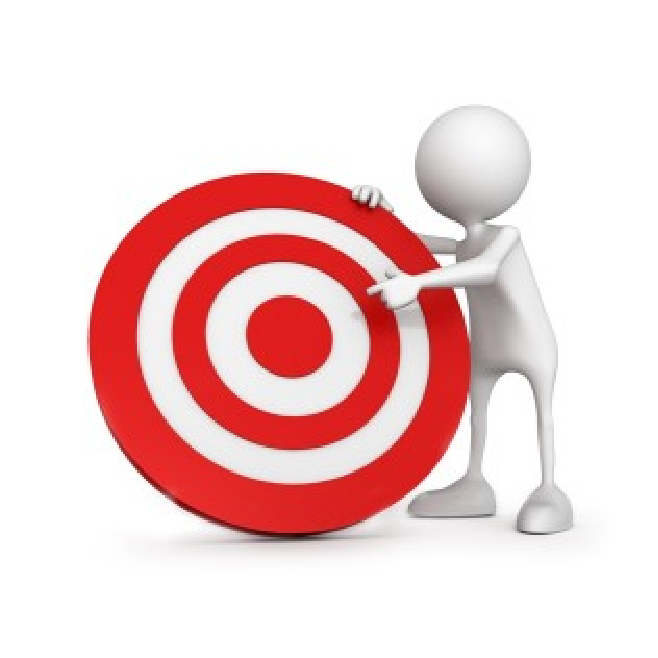
\includegraphics[scale=0.4]{figuras/objective.eps}
\end{figure}

\end{frame}

\subsection{Objetivos Específicos}

\begin{frame}
\frametitle{Objetivos Específicos}

\begin{itemize}
	\item \textbf{Aprofundar os conhecimentos em termos de redes sociais} e afins, através da leitura de materiais bibliográficos.
	\item Definir uma arquitetura com base no \textbf{uso de grafos}, alinhada às boas práticas da Engenharia de Software, para representar os relacionamento entre as pessoas bem como as rotas percorridas por elas.
	\item Evoluir a arquitetura proposta, visando lidar com \textbf{algoritmos para compatibilizar agendas entre os interessados}.
\end{itemize}

\end{frame}

\begin{frame}
\frametitle{Objetivos Específicos}

\begin{itemize}
	\item \textbf{Usar estruturas de dados e algoritmos específicos}, implementados de forma otimizada, visando \textbf{desempenho e facilidades na manutenção evolutiva do software}.
	\item \textbf{Instanciar um produto de software} - i.e. uma rede social específica - a partir do \textit{framework}, no intuito de coletar as primeiras impressões acerca do suporte desenvolvido como tema foco desse trabalho.
	\item Orientar-se por uma \textbf{metodologia que permita trabalhar a investigação do domínio de redes sociais}, a identificação de suporte tecnológico adequado, o desenvolvimento do \textit{framework}, a instanciação do mesmo, e a coleta das primeiras impressões com base nos resultados obtidos.
\end{itemize}

\end{frame}

\section{Metodologia}

\begin{frame}
\frametitle{Fluxo Geral de Trabalho}

\begin{figure}[h]
	\centering
	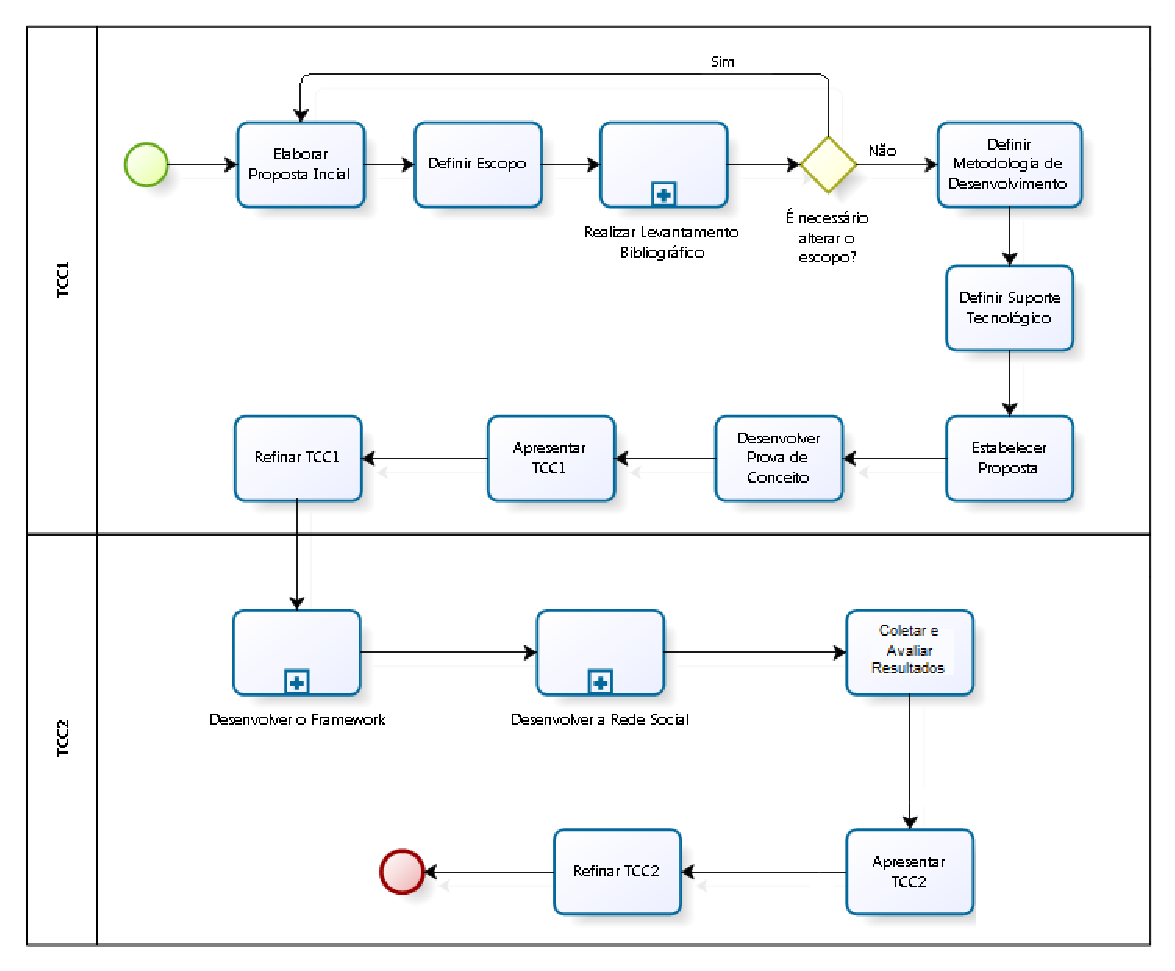
\includegraphics[scale=0.45]{../figuras/capitulo2/processo_tcc.eps}
\end{figure}

\end{frame}

\begin{frame}
\frametitle{Metodologia de Desenvolvimento}

Práticas ágeis baseadas no SCRUM e XP;

\begin{itemize}
	\item Pareamento;
	\item Estórias de usuário;
	\item Backlog;
	\item Planning poker;
	\item Sprints;
\end{itemize}

\begin{figure}[h]
	\centering
	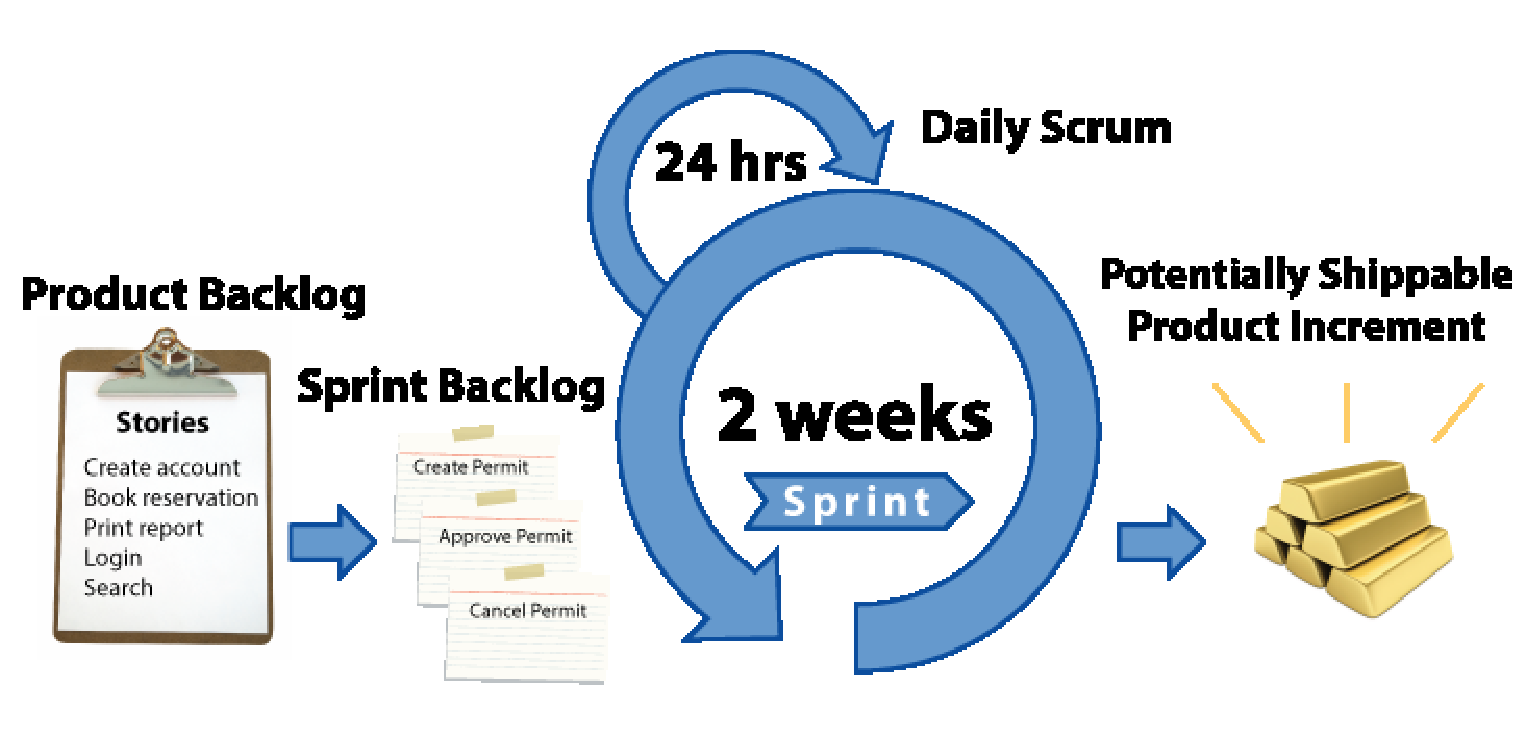
\includegraphics[scale=0.3]{figuras/scrum.eps}
\end{figure}

\end{frame}

\begin{frame}
\frametitle{Fluxo de Desenvolvimento}

\begin{figure}[h]
	\centering
	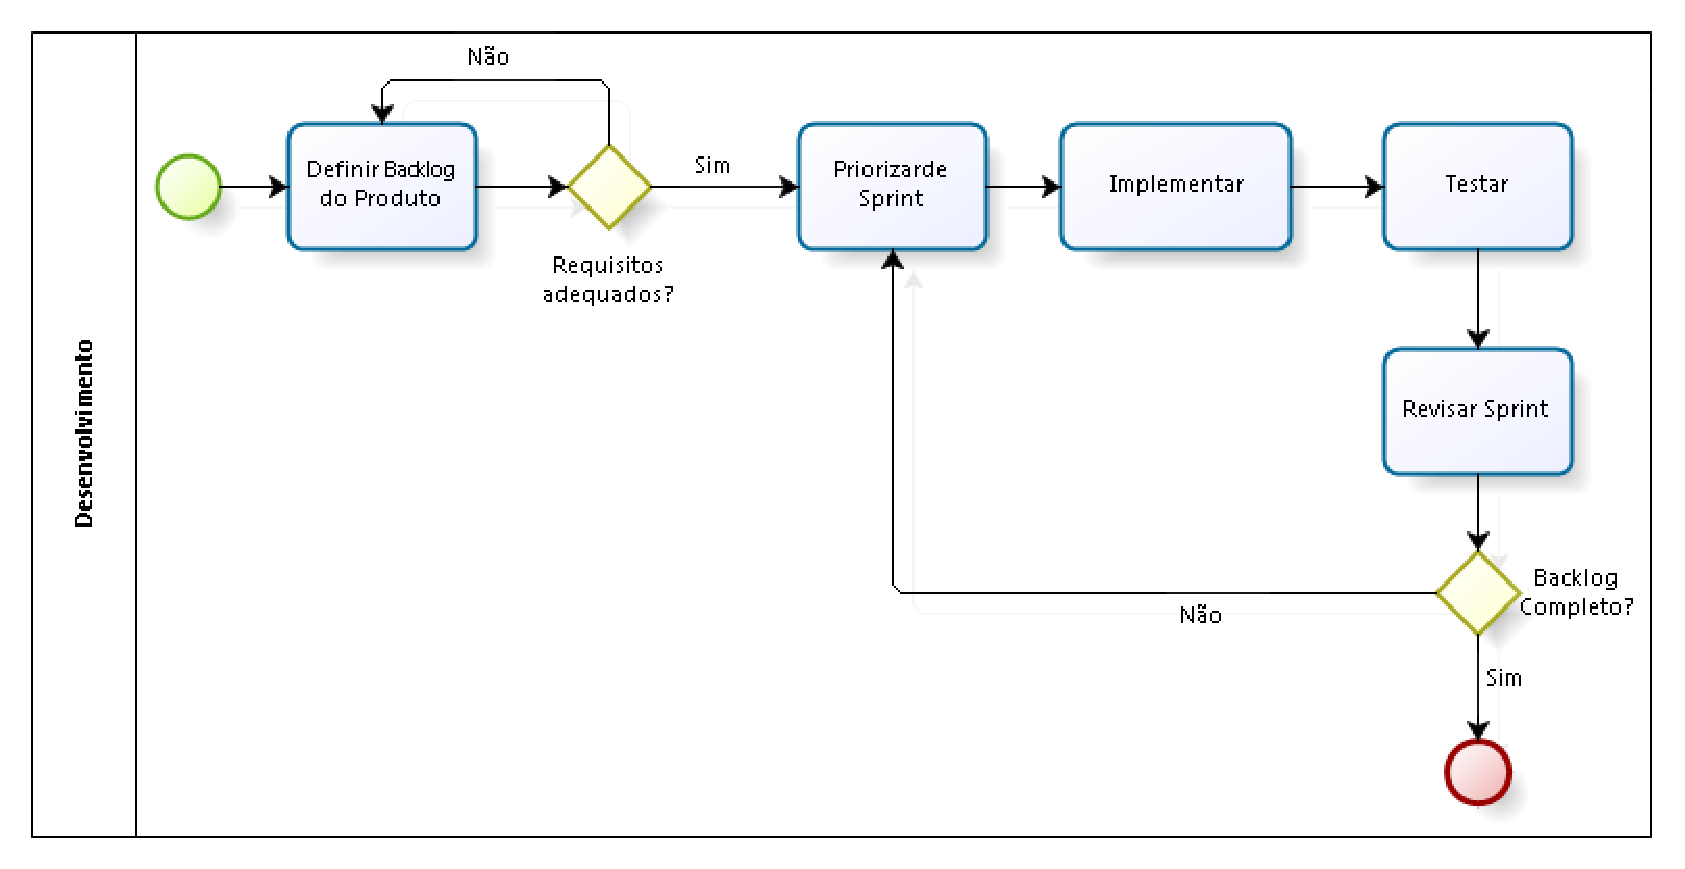
\includegraphics[scale=0.35]{../figuras/capitulo2/processo_desenvolvimento.eps}
\end{figure}

\end{frame}

\section{Proposta}

\begin{frame}
\frametitle{O Framework}

\begin{itemize}
	\item Recursos de rotas;
	\item Recursos de agendas;
	\item Recursos gerais;
	\item Caixa cinza;
	\item Extensível, com pontos flexíveis;
	\item Tecnologia Ruby on Rails.
\end{itemize}

\begin{figure}[h]
	\centering
	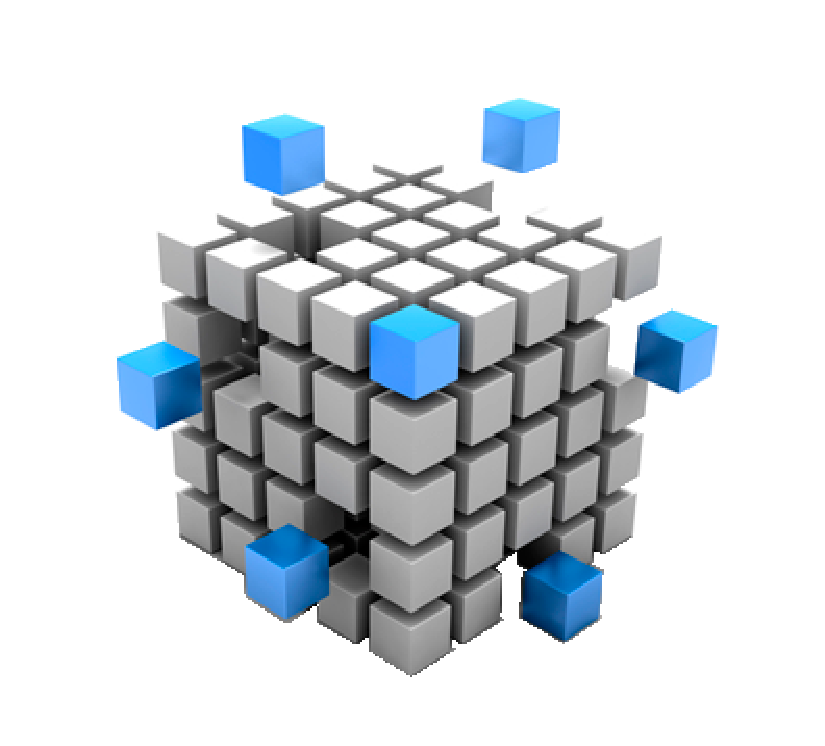
\includegraphics[scale=0.35]{figuras/framework.eps}
\end{figure}

\end{frame}

\begin{frame}
\frametitle{Tipos de Relacionamentos}

\begin{figure}[h]
	\centering
	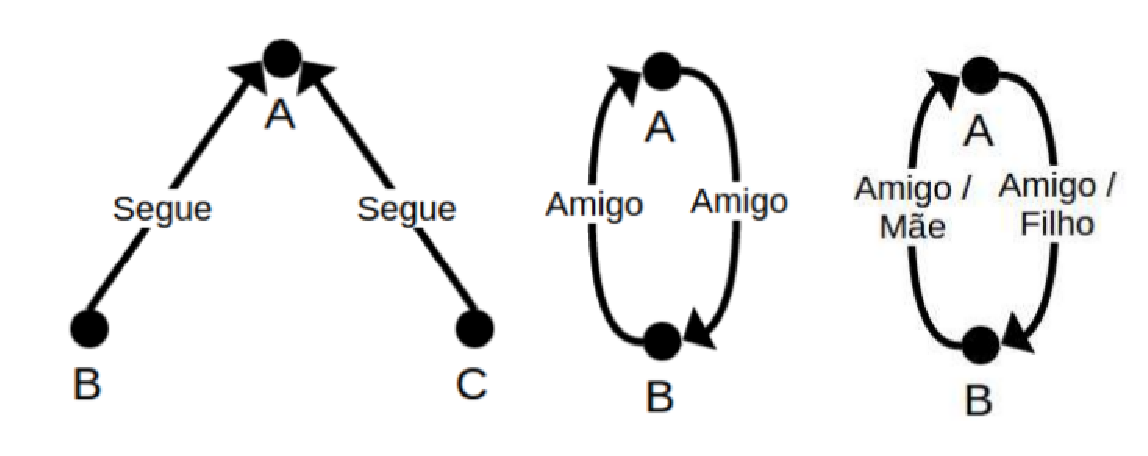
\includegraphics[scale=0.6]{figuras/relacionamentos.eps}
\end{figure}

\end{frame}

\begin{frame}
\frametitle{Rotas}

\begin{itemize}
	\item Definição de rotas;
	\item Compatibilidade de rotas;
\end{itemize}

\begin{figure}[!h]
	\centering
	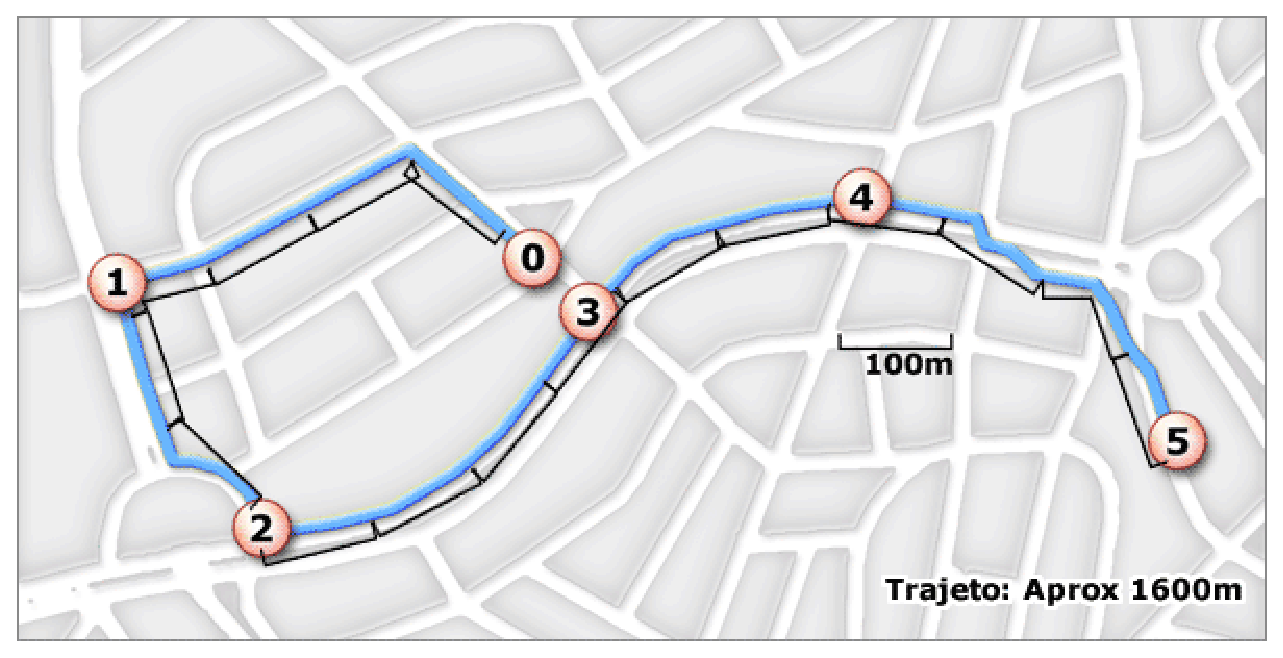
\includegraphics[scale=0.4]{../figuras/capitulo3/rota.eps}
	\caption[Exemplo de rota]{Exemplo de rota\footnotemark}
	\label{rota}
\end{figure}
\footnotetext{\url{http://sede.wikidot.com/andy-s-brainstorm}}

\end{frame}

\begin{frame}
\frametitle{Agendas}

\begin{itemize}
	\item Criação de agendas;
	\item Marcação de eventos;
	\item Compatibilidade de horários;
\end{itemize}

\begin{figure}[h]
	\centering
	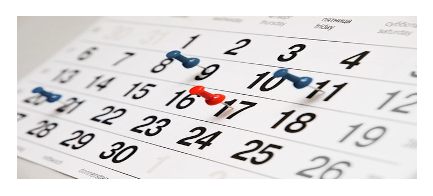
\includegraphics[scale=0.8]{figuras/scheduler.eps}
\end{figure}

\end{frame}

\begin{frame}
\frametitle{Uso do Framework}

\begin{itemize}
	\item Instanciação do \textit{framework};
	\item Disponibilização de \textit{hotspots};
	\item Indicação de uso de serviços \textit{RESTFul};
\end{itemize}

\end{frame}

\begin{frame}
\frametitle{Uso do Framework}

\begin{figure}[!h]
	\centering
	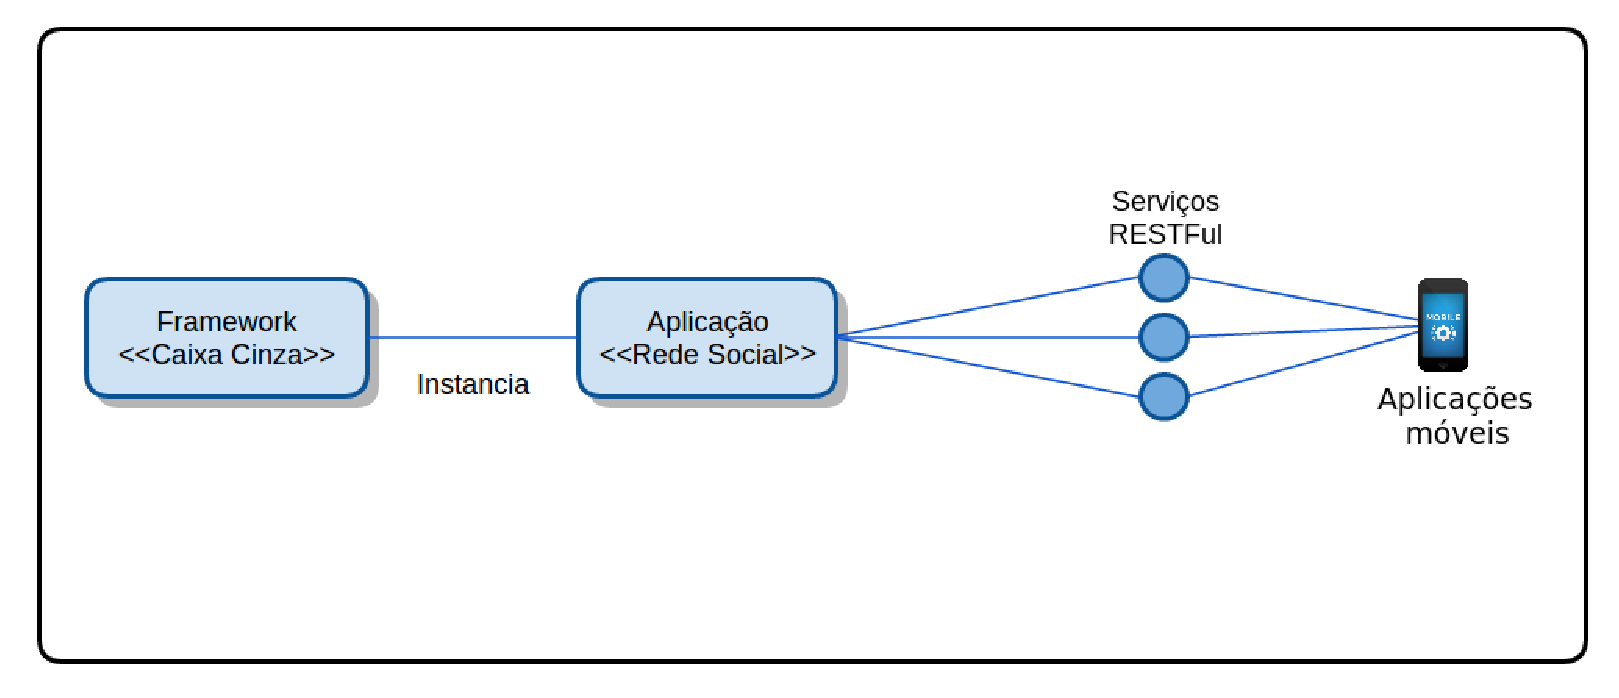
\includegraphics[scale=0.45]{../figuras/capitulo3/uso_proposto.eps}
	\caption{Modelo ilustrando um possível uso do \textit{Framework}}
	\label{uso_proposto}
\end{figure}

\end{frame}

\begin{frame}
\frametitle{Prova de Conceito}

\begin{itemize}
	\item Verificar viabilidade do tema;
	\item Apresentar inicialmente alguns recursos de software;
	\item Usuários;
	\item Arestas;
	\item Rede;
	\item Buscas no grafo.
\end{itemize}

\begin{figure}[h]
	\centering
	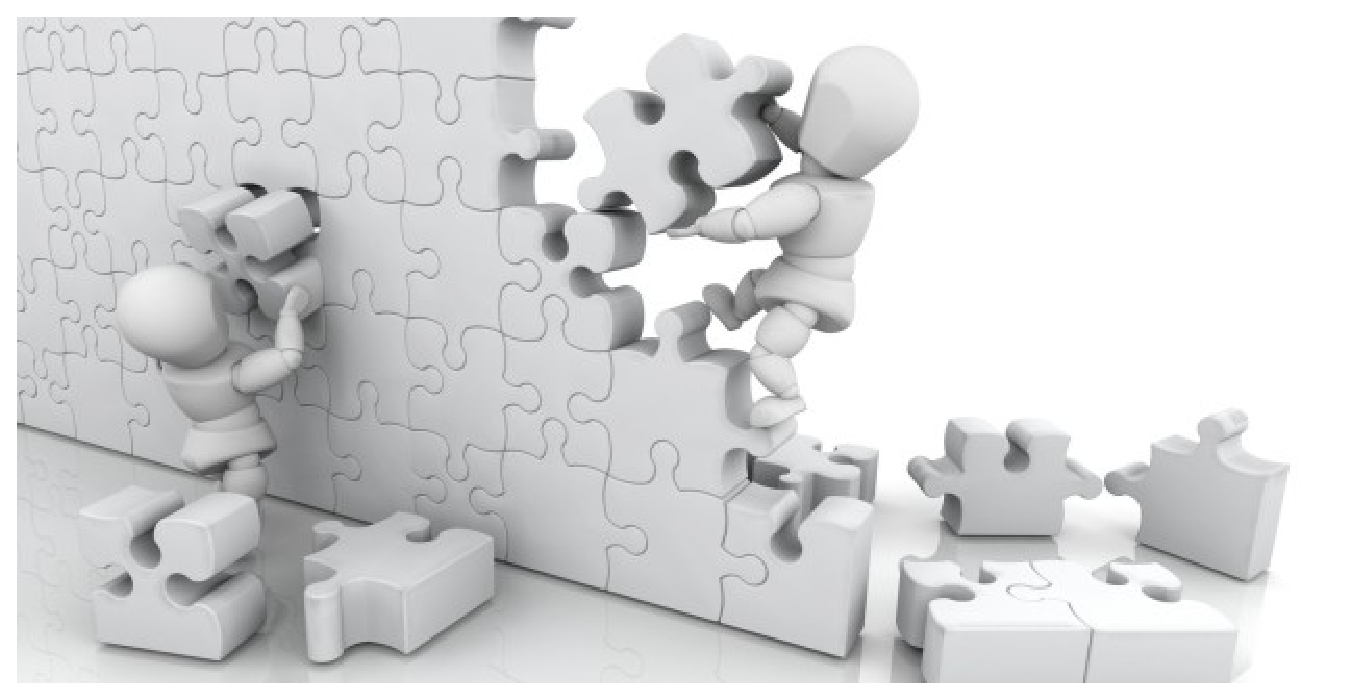
\includegraphics[scale=0.3]{figuras/concept-test.eps}
\end{figure}

\end{frame}

\begin{frame}
\frametitle{Próximas etapas}

\begin{itemize}
	\item Definição de backlog do produto;
	\item Definição e priorização de sprints;
	\item Desenvolvimento do framework;
	\item Desenvolvimento da rede social;
\end{itemize}

\begin{figure}[h]
	\centering
	
\includegraphics[scale=0.15]{figuras/future.eps}
\end{figure}

\end{frame}

\begin{frame}
\Huge{\centerline{Obrigado!}}
\end{frame}

\begin{frame}
\frametitle{Referências}
\footnotesize{
\begin{thebibliography}{99} % Beamer does not support BibTeX so references must be inserted manually as below
\bibitem[Krueger, 1992]{krueger} Krueger, Charles W. (1992)
\newblock Software Reuse
\bibitem[Marteleto, 2001]{marteleto} Marteleto, Regina Maria (2001)
\newblock Mídias Sociais: uma contribuição de análise
\end{thebibliography}
}
\end{frame}

\end{document} 